\documentclass[12pt]{article}
	\usepackage{graphicx,amsmath}
	\usepackage[round]{natbib}
	\linespread{1.3}
	\bibliographystyle{plainnat}
	\title{
		Group \#07 \\
		Bridge-00 \\
		18g, 1700N \\[1cm]
		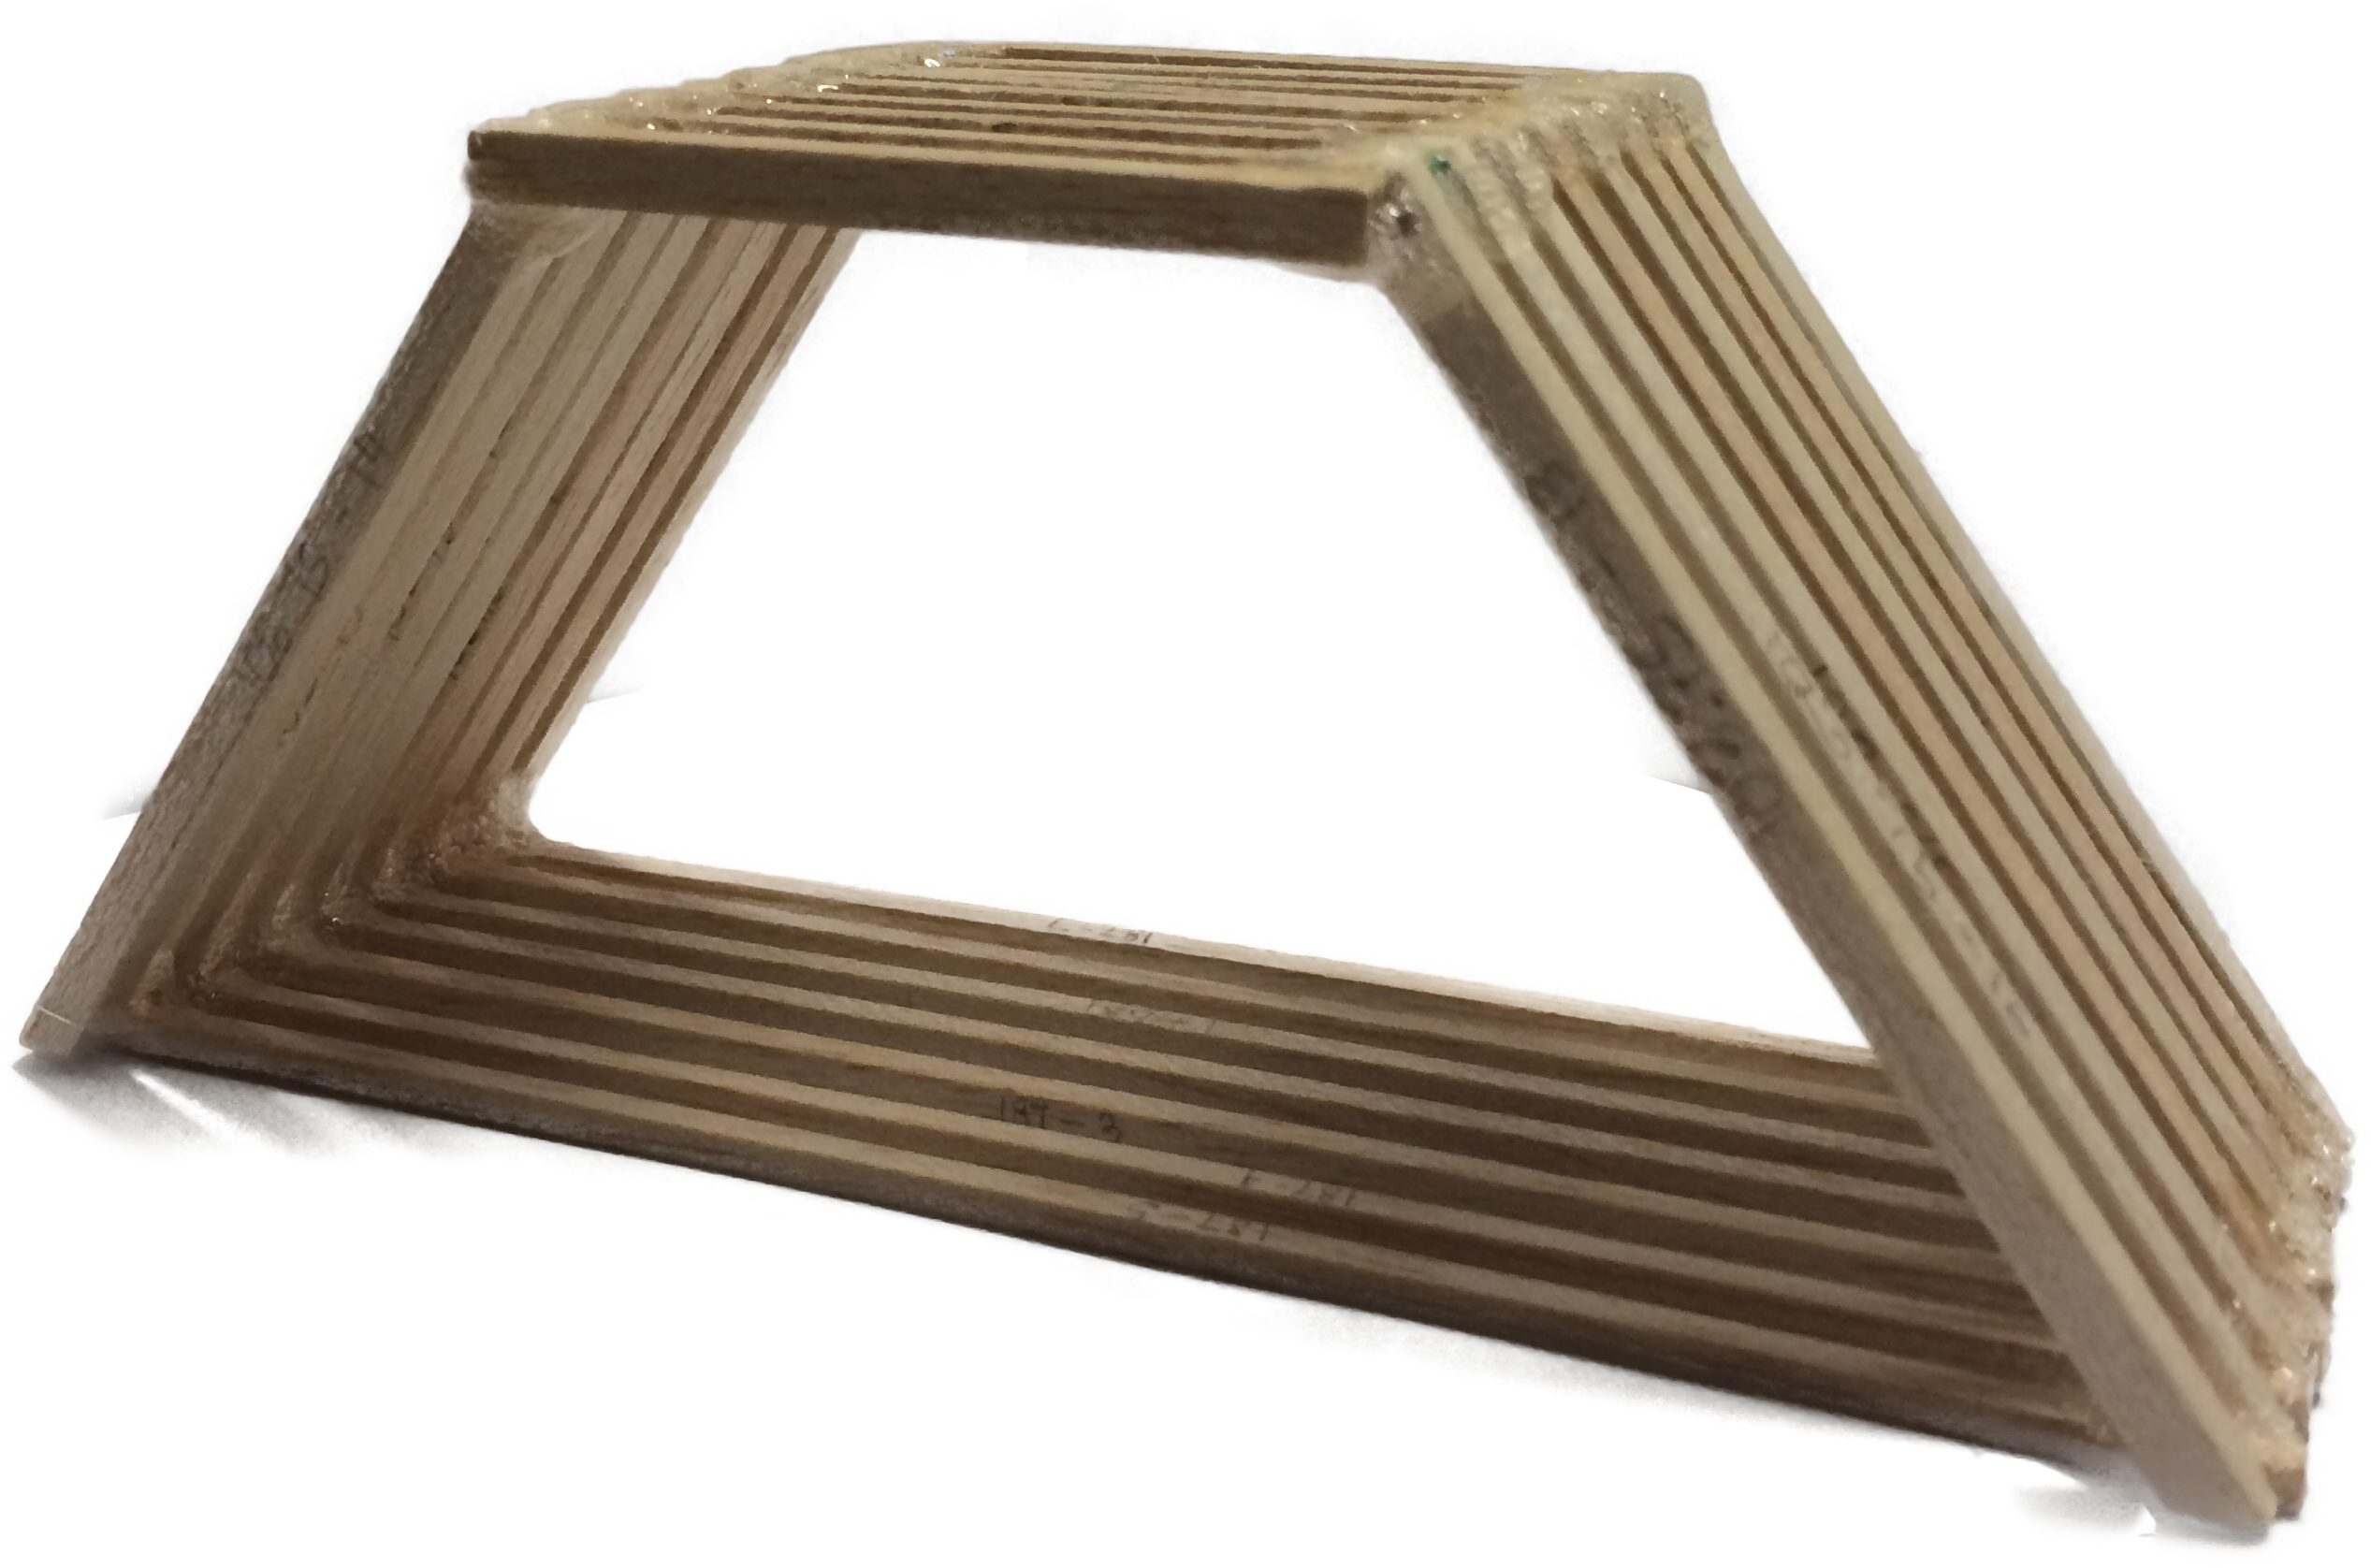
\includegraphics[width=0.7\textwidth]{photo}
	}
	\author{
		Alex Miles \\ u5568175 \\ 16.7\%
		\and Arlene Mendoza \\ u5589650 \\ 16.7\%
		\and Itsuki Nishida \\ u5578430 \\ 16.7\%
		\and Paul Apelt \\ u5568225 \\ 16.7\%
		\and Stephen Lonergan \\ u5349877 \\ 16.7\%
		\and Thomas Hale \\ u5568225 \\ 16.7\%
	}
\begin{document}
	\maketitle
	\section{Design}
		% design assumptions and methods
		\subsection{Assumptions}
		During the design process, the following assumptions have been made \citep[p.~264]{tbook}:
		\begin{enumerate}
			\item All loadings are applied at the joint,
			\item Weight of the members neglected,
			\item Joints are smooth (friction-less) pins,
			\item Each member has no more than two joints.
		\end{enumerate}
		% TODO: why trapezium
		% other designs considered
		% photo of a prototype
		Final bridge design can be seen in Figures \ref{dim} and \ref{proj}.
		\begin{figure}[h!]
			\centering
			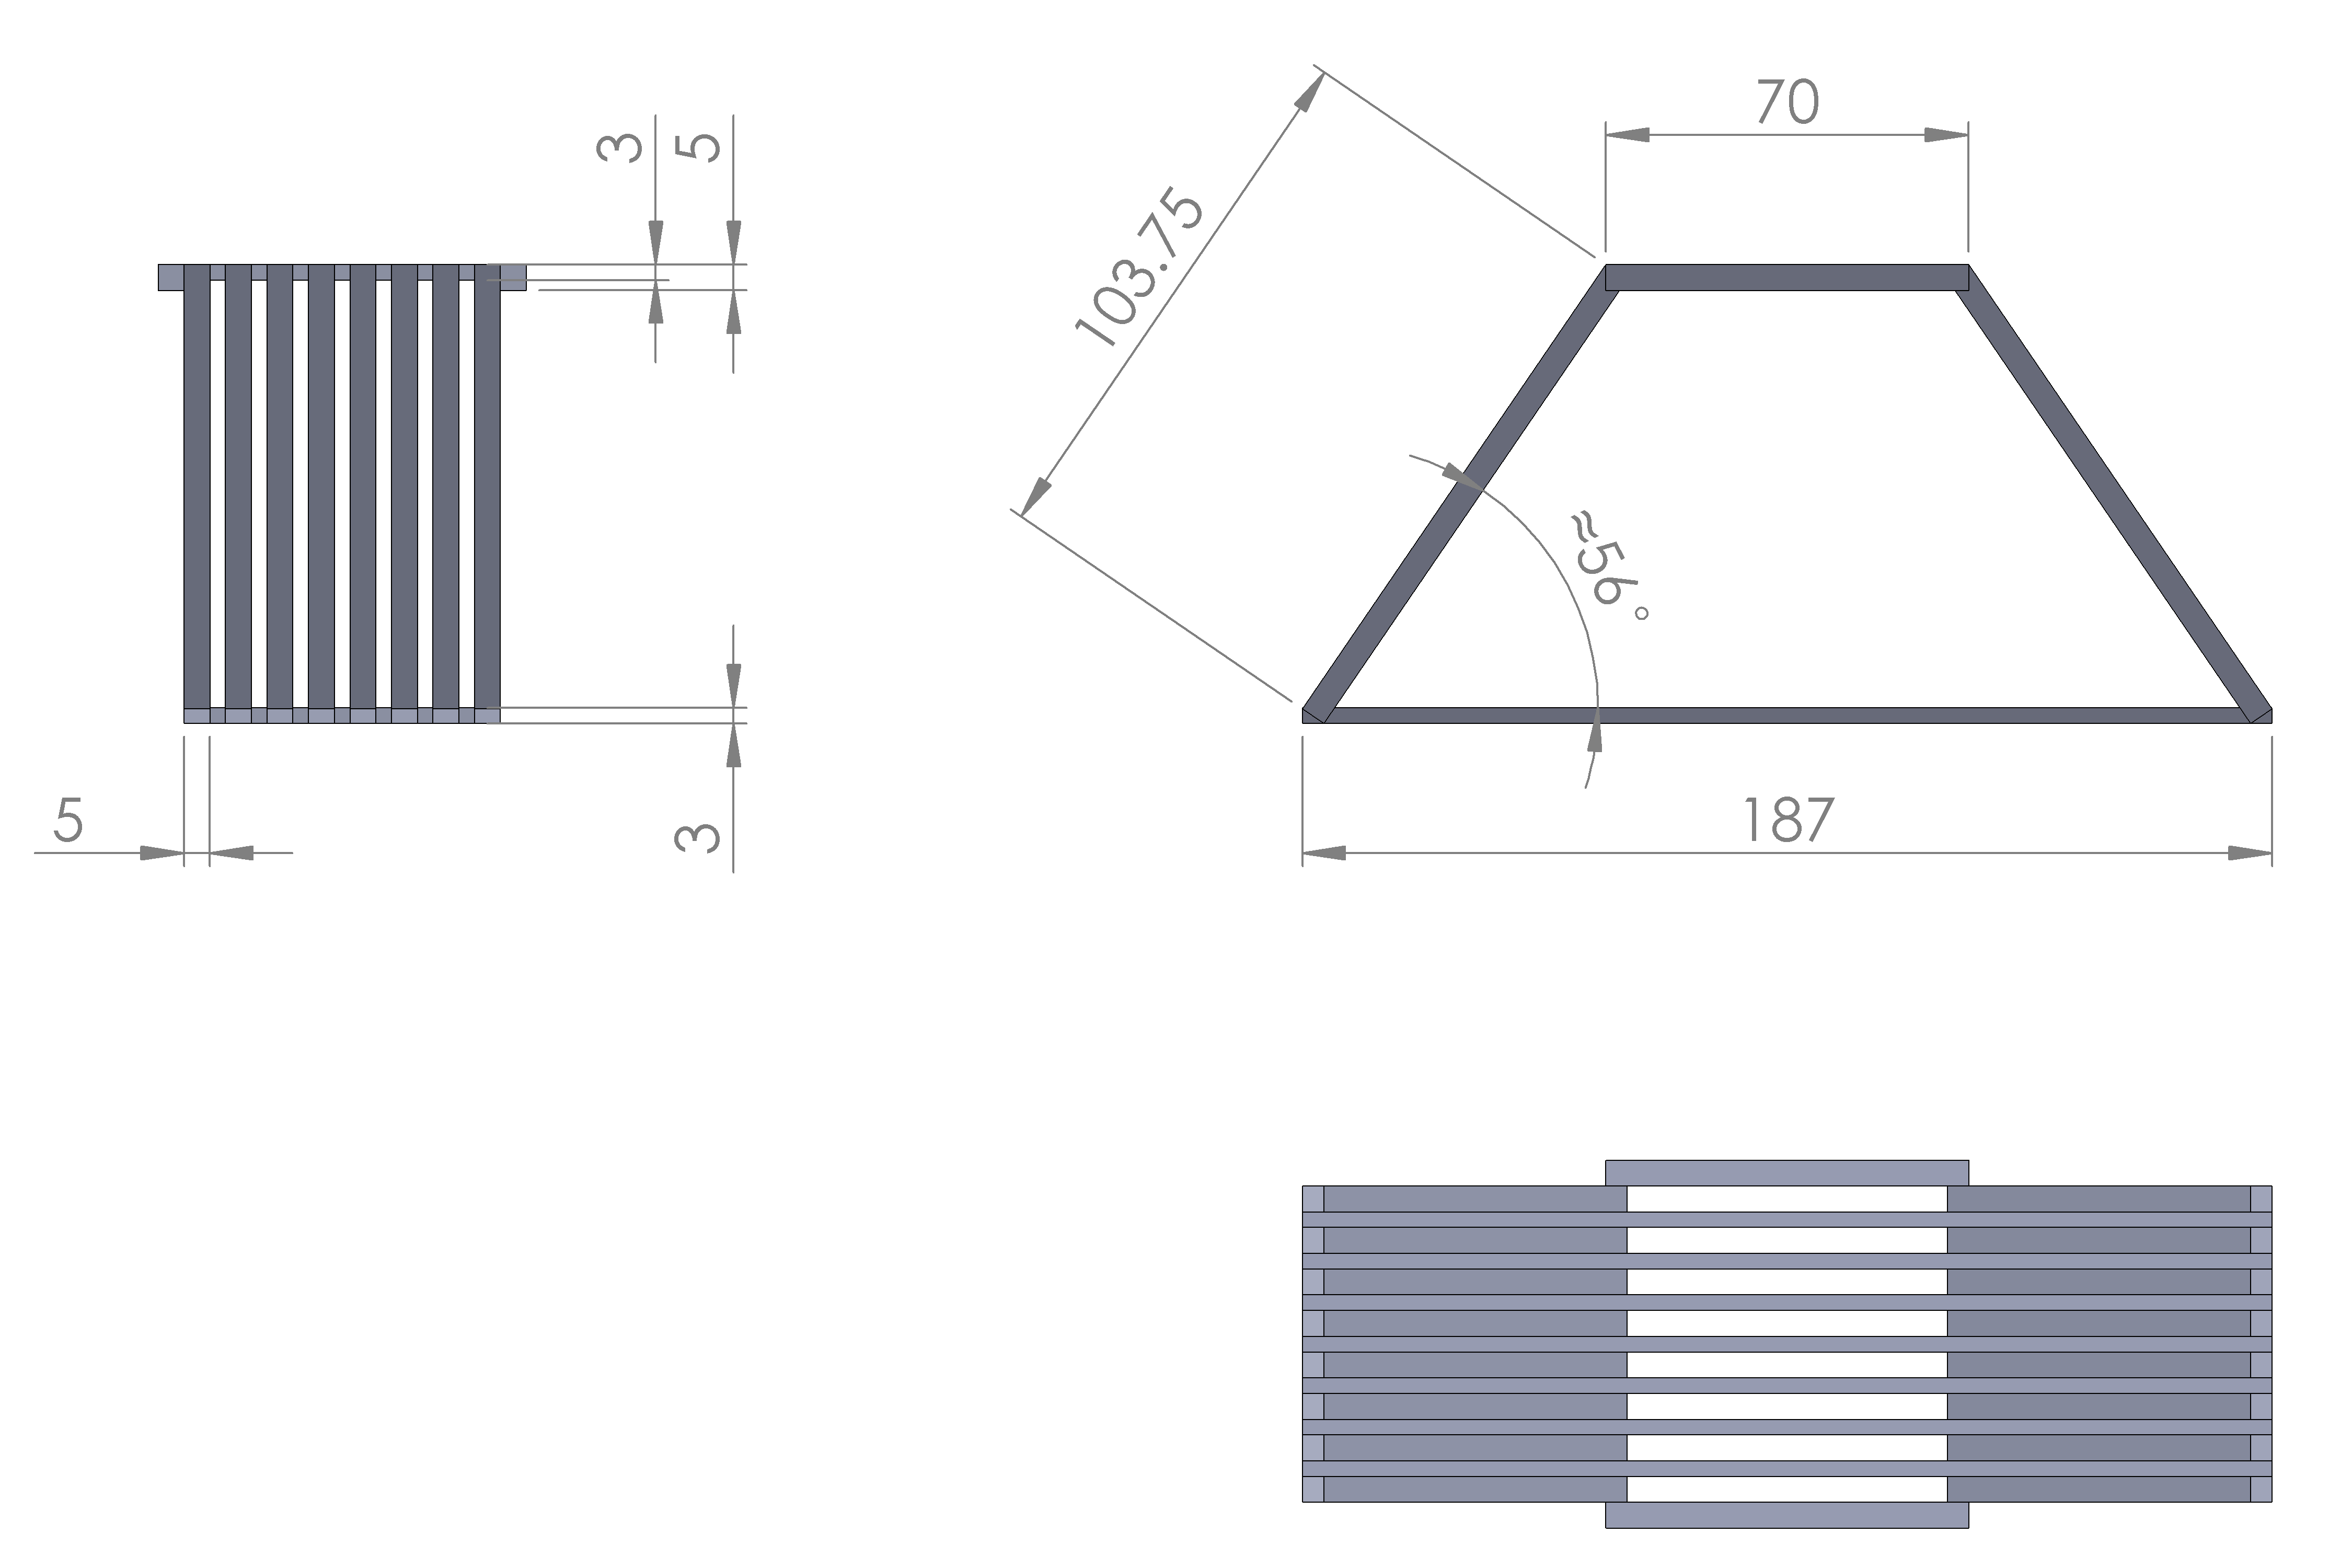
\includegraphics[width=\textwidth]{dim}
			\caption{Dimensioned drawing.}
			\label{dim}
		\end{figure}
		\begin{figure}[h!]
			\centering
			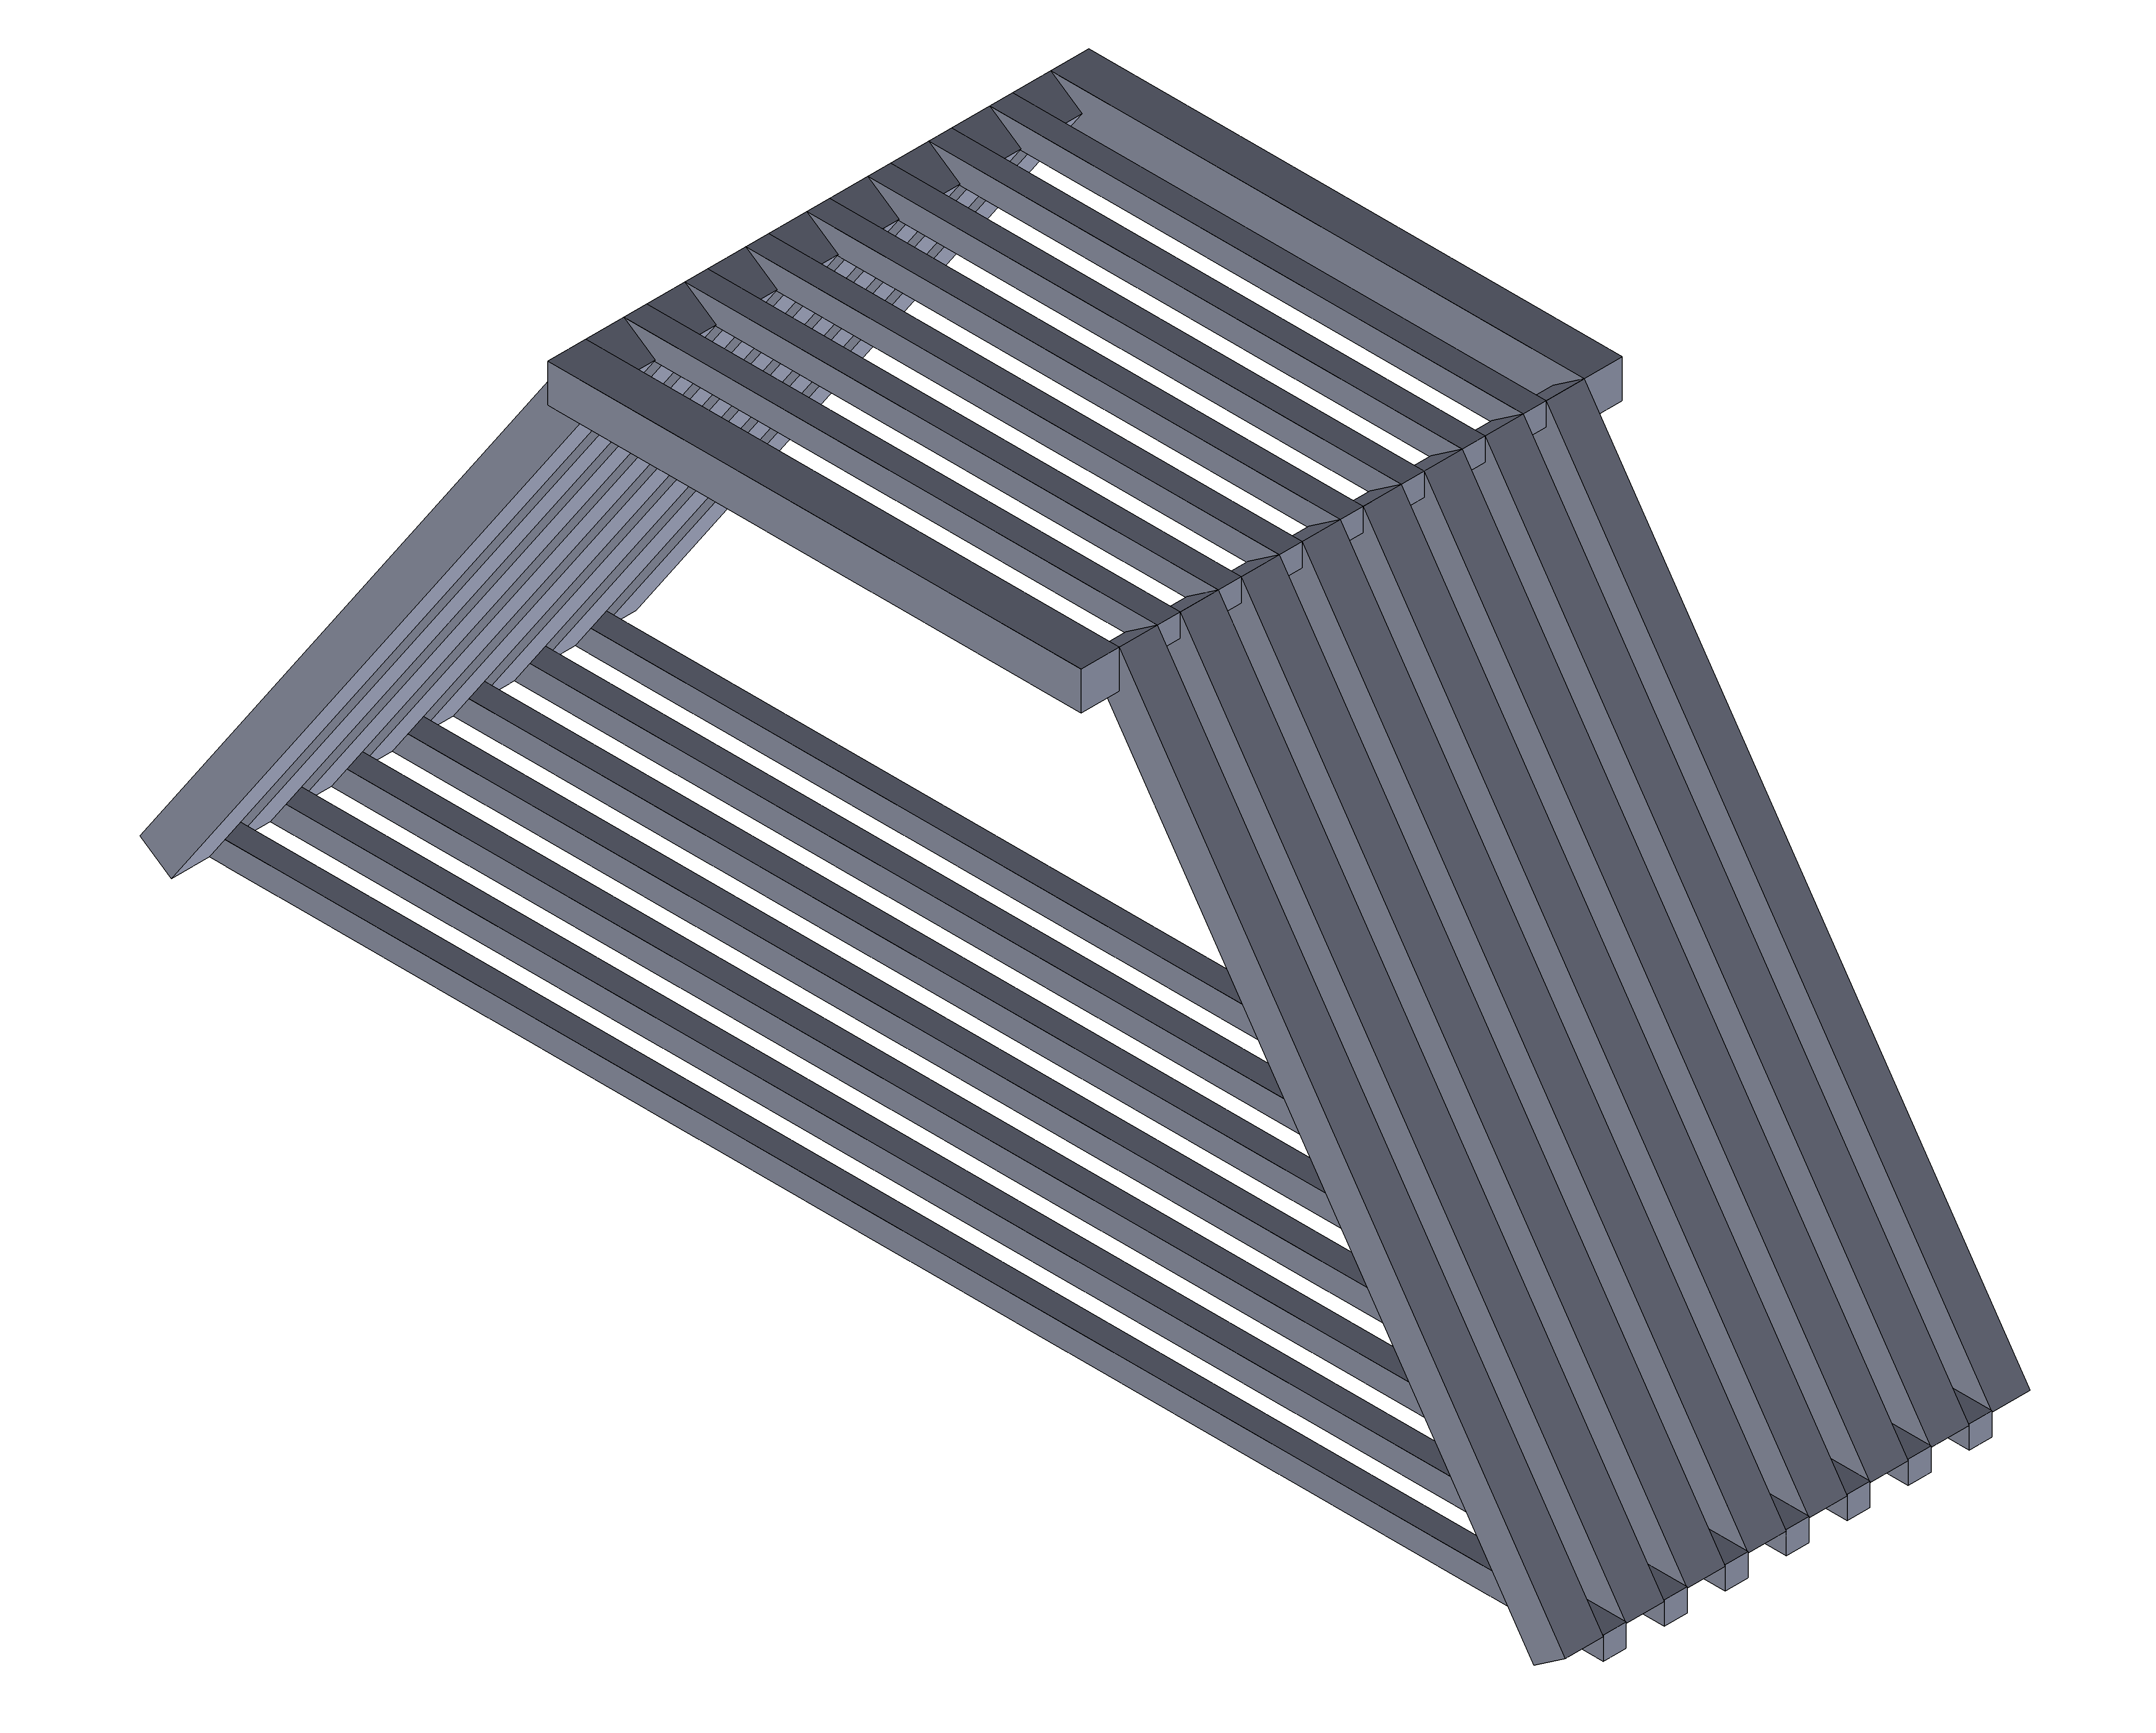
\includegraphics[width=0.6\textwidth]{proj}
			\caption{3D-Projection.}
			\label{proj}
		\end{figure}
		% dimensioned drawing
		\subsection{Methods}
		% construction process 
		% materials Used
		% difficulties faced - measuring accurately, It ended up being 185mm than 187mm and the trapezium was also slightly lopsided by a 1mm, angles are fucked!
		% weight issues - excess glue fail 
		% picture of the materials used
	\section{Analysis}
		Due to the unconventional design, to ease the calculations during the analysis, it was assumed that the load is equally distributed between eight trapezium-shaped trusses. Thus, a single trapezium truss was analyzed, and then extended to approximate the entire bridge. Internal forces, nodes and members are labelled as per Figure~\ref{trap}. As the truss is symmetrical, only two nodes needed to be analyzed.
		\begin{figure}[h!]
			\centering
			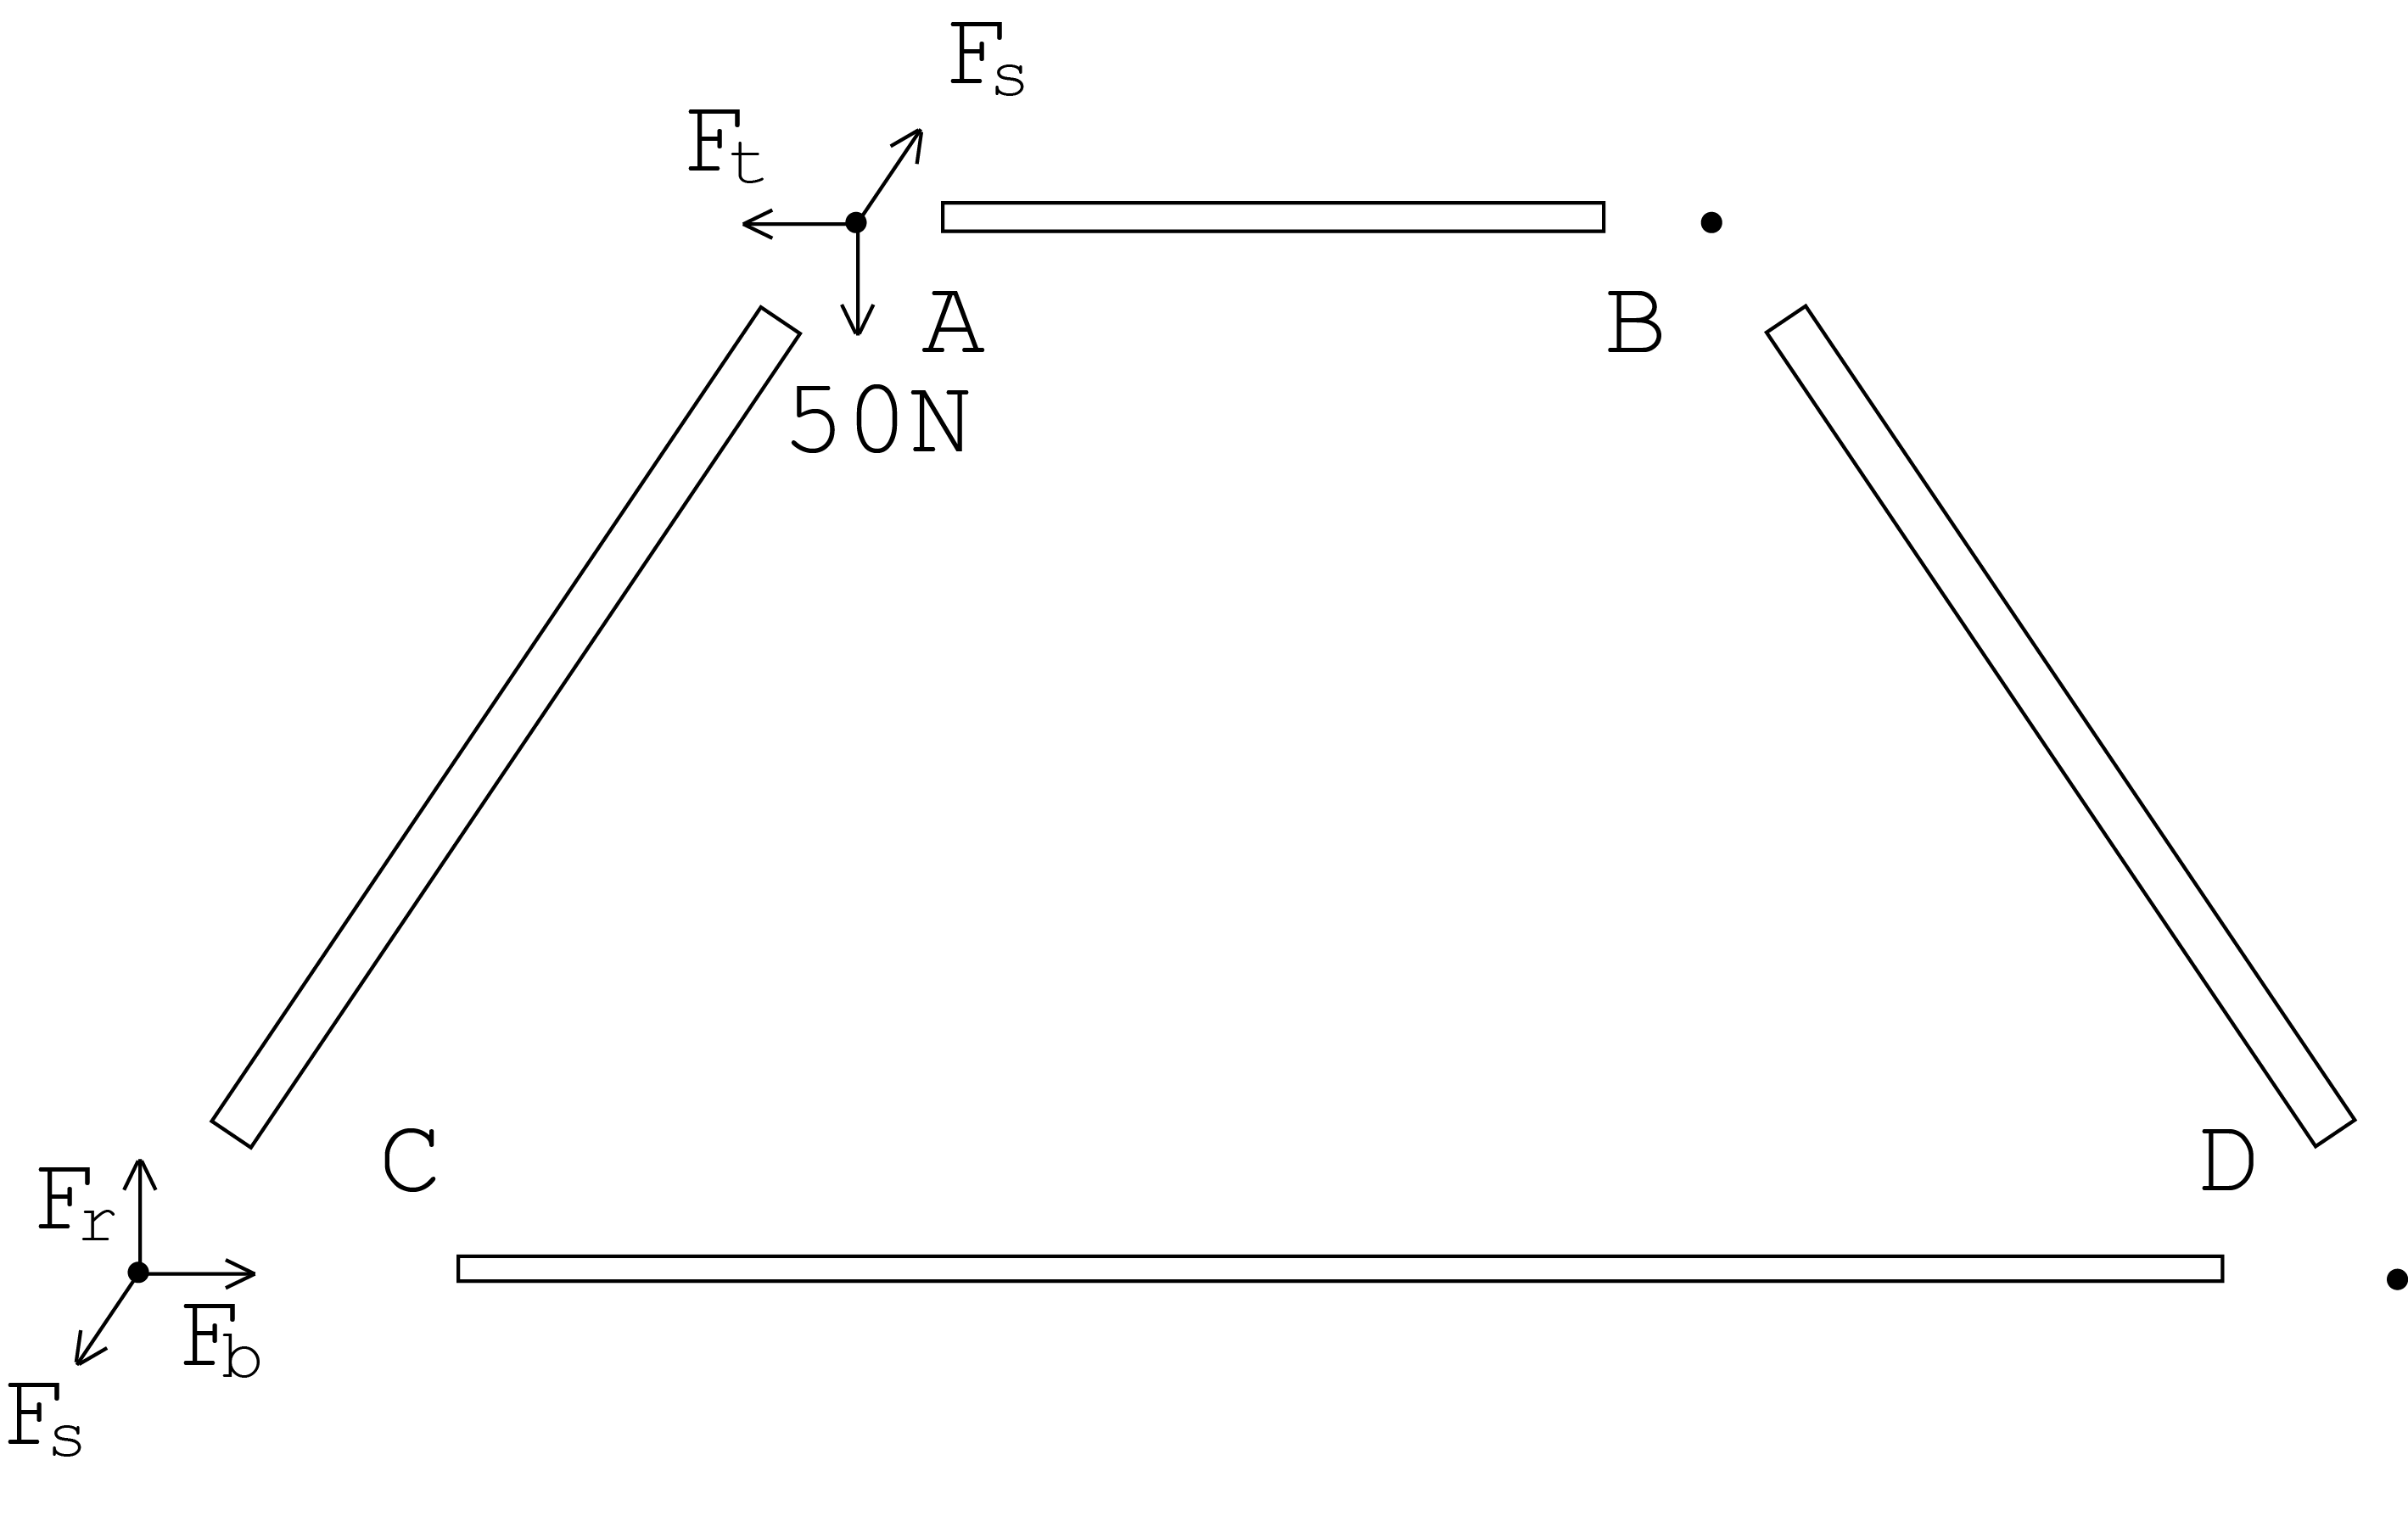
\includegraphics[width=0.8\textwidth]{trapanal}
			\caption{Trapezium truss.}
			\label{trap}
		\end{figure}
		For a load of 100N divided equally between nodes A and B, force equilibrium for nodes A and C are described in equation blocks \ref{eqn1} and \ref{eqn2} respectively.
		% insret calculations here
		\begin{subequations}
			\begin{align}
				F_s \sin 56&=50\mathrm{N}, \\
				F_s \cos 56&=F_t.
			\end{align} \label{eqn1}
		\end{subequations}
		\begin{subequations}
			\begin{align}
				F_s \sin 56&=F_r, \\ 
				F_s \cos 56&=F_b.
			\end{align} \label{eqn2}
		\end{subequations}
		The results of solving the above equations are presented in Table~\ref{loads}. Note that the internal force experienced by members is twice the given value, because it occurs at both ends.
		% table of member loads
		\begin{table}[h!]
			\caption{Member loads.}
			\begin{center}
			\begin{tabular}{ | r | l | }
				\hline
				70 3x3 mm (top) & 33.7 N (c) \\ \hline
				103.75 5x5 mm (side) & 60.3 N (c) \\ \hline
				187 3x3 mm (bottom) & 33.7 N (t) \\ \hline
			\end{tabular}
			\end{center}
			\label{loads}
		\end{table}
		% assumptions
		% max load
		Maximum loads for each member were calculated using the values given in the Assignment sheet. Modulus of elasticity $E=3\mathrm{GN}/\mathrm{m}^2$, standard deviation $\sigma=+2.4/-2.1\mathrm{MN}/\mathrm{m}^2$. Tensile strength $\sigma_t=20\mathrm{GN}/\mathrm{m}^2$,  standard deviation $\sigma=+3.6/-3.4\mathrm{MN}/\mathrm{m}^2$. Compressive strength $\sigma_t=12\mathrm{GN}/\mathrm{m}^2$,  standard deviation $\sigma=+2.1/-2.8\mathrm{MN}/\mathrm{m}^2$. To calculate maximum load from strength values, equation \ref{eqs} was used. The results are presented in Table~\ref{maxloads}.
		\begin{equation}
			\sigma=\frac{P}{A}
			\label{eqs}
		\end{equation}
		\begin{table}[h!]
			\caption{Maximum member loads.}
			\begin{center}
			\begin{tabular}{ | r | l | l | }
				\hline
				& average & $-1\sigma$ \\ \hline
				3x3 mm (c) & 108 N & 82.8 N \\ \hline
				3x3 mm (t) & 180 N & 149.4 N \\ \hline
				5x5 mm (c) & 300 N & 230 N \\ \hline
			\end{tabular}
			\end{center}
			\label{maxloads}
		\end{table}
		% TODO: add buckling
		% reasons
		To predict the maximum load, the weakest section of the bridge had to be found. That was done by first summing up the maximum loads of all top, bottom and side members, (equation block~\ref{eqsa}), using values from Table~\ref{maxloads}, average column.
		\begin{subequations}
			\begin{align}
				P_{top}&=7\times108+2\times300
				&=1356\mathrm{N}\\
				P_{side}&=8\times300
				&=2400\mathrm{N}\\
				P_{bottom}&=7\times180
				&=1260\mathrm{N}
			\end{align}
			\label{eqsa}
		\end{subequations}
		Then the safety rations (defined in equation~\ref{eqr}) were calculated for each section (equation block~\ref{eqrl}), using values from Table~\ref{loads}.
		\begin{equation}
			R=\frac{P_{max}}{P}
			\label{eqr}
		\end{equation}
		\begin{subequations}
			\begin{align}
				R_{top}&=40.2\\
				R_{side}&=39.8\\
				R_{bottom}&=37.4
			\end{align}
			\label{eqrl}
		\end{subequations}
		The lowest safety ratio member will break first, thus bottom was determined to be the breaking point. The actual maximum load was determined in equation block~\ref{eqt}, where $P$ is the load used to calculate $R$. The same steps were carried out in equation block~\ref{eqs}, but the strength was assumed to be $1\sigma$ below average.
		\begin{subequations}
			\begin{align}
				F&=\frac{R P}{2} \\
				&=1869.4
			\end{align}
			\label{eqt}
		\end{subequations}
		\begin{subequations}
			\begin{align}
				F&=\frac{R_{\sigma} P_{\sigma}}{2} \\
				&=1551.6
			\end{align}
			\label{eqs}
		\end{subequations}
		The average of the two $1710.5\mathrm{N}$, was chosen as predicted maximum load.
	\section{Results}
		% analysis of the difference
		% why fail
		% much sad
		% testing machine OP
		% please nerf
		%Add pic of the final bridge and show the glue
		%What was the final load it could hold?
	\bibliography{bib}
\end{document}

